\setchapterimage[6cm]{chapter/human_settlement/human_settlement_main.jpg}
%\setchapterstyle{kao}
\setchapterpreamble[u]{\margintoc}
\chapter[In which settlements of Russia are more scientists born, rural or town?]{In which settlements of Russia are more scientists born, rural or town?\protect\footnotemark}
\labch{human_settlement}

\footnotetext{\href{https://commons.wikimedia.org/wiki/File:Detail_of_the_settlement_Vestmannaeyjar-2.jpg}{Human settlement}. 
	Author: \href{https://commons.wikimedia.org/wiki/File:Detail_of_the_settlement_Vestmannaeyjar-2.jpg}{Szilas / 2014 /  Creative Commons Attribution License}.}

The chapter explores the Wikidata object, \wdqName{human settlement}{486972} settlement and its properties. In each of the sections, 
tasks are presented that were solved using SPARQL queries.

A list of settlements was received,
bubble charts were built with the number of population in ``human settlement'' by country.
A chart showing the proportion of the population
living in settlements relative to the entire population of the country.
The chart showed that a high percentage of the population living in localities
falls in agricultural countries, while in more industrialized countries
a smaller proportion of the population lives in human settlement.

To compare rural and town settlements
built diagrams of the number of scientists, grouped by occupation
and divided by place of birth: rural or town.

To search for more complete answers to the above tasks
more general classes were found for the object \wdqName{human settlement}{486972}
using the property \wdProperty{31}{instance of}.
The difficulty of the study is due to the lack of a clear typology of human settlements
(for example, from population size) in Russian legislation and in Wikidata.

%%%%%%%
\section{List of ``human settlement''}

Let's build a list of all human settlements using the query~\ref{lst:human-settlement1} \footnote{List of all human settlements. \num{411393} items received in 2017. SPARQL query:\href{https://w.wiki/4f2\$}{https://w.wiki/4f2\$}}.

\begin{lstlisting}[ language=SPARQL, 
                    label=lst:human-settlement1,
                    texcl 
                    ]
# List of all human settlements
SELECT ?hum ?humLabel WHERE{
  ?hum wdt:P31 wd:Q486972. # instance of human settlement
  SERVICE wikibase:label{bd:serviceParam wikibase:language "en"}
}
\end{lstlisting}%

In 2021, it turned out to be impossible to get a list of human settlements
due to the large number of objects and, therefore, the query takes too long~\ref{lst:human-settlement1}.
To calculate the number of all human settlements, refer to the \lstinline|COUNT()|
in the request~\ref{lst:human-settlement2}.

\index{SPARQL!COUNT!Number of human settlements}
\begin{lstlisting}[ language=SPARQL, 
                    caption={Number of human settlements. \num{411393} items received in 2021. SPARQL query:\href{https://w.wiki/4d7s}{https://w.wiki/4d7s}},
                    label=lst:human-settlement2,
                    texcl 
                    ]
# Number of human settlements
SELECT (COUNT(?hum) AS ?count) WHERE {
  ?hum wdt:P31 wd:Q486972. # instance of human settlement  
}
\end{lstlisting}%

Among domestic settlements on Wikidata,
which correspond to the articles of the Russian Wikipedia,
almost empty are, for example,
former village \wdqName{Borisovo}{4093951} (3 properties)
and \wdqName{Brigadier forestry}{21668554} (4 properties).

According to the ProWD service
among domestic settlements
\wdqName{Yalta}{128499} has the most properties (36).
The world leader is \wdqName{Tokyo}{1490} (73 properties)\sidecite{humansettlements_ProWD}.

%%%%%%%
\section{List of countries by total population}

Using the query~\ref{lst:human-settlement3}
Let's build an ordered list of countries according to the total number of people living in ``human settlement''.

\index{SPARQL!SUM!List of countries by population in ``human settlement''}
\index{SPARQL!GROUP BY!List of countries by population in ``human settlement''}
\lstset{numbers=left, firstnumber=1, frame=single}
\begin{lstlisting}[ language=SPARQL, 
    caption={List of countries by population in settlements. The result contained \num{161} countries in 2017 and \num{213} countries in 2021. SPARQL query:\href{https://w.wiki/4f35}{https://w.wiki/4f35}},
    label=lst:human-settlement3,
    texcl 
                  ]
# List of countries by population in settlements
SELECT ?country ?countryLabel (SUM(?population) as ?sumPopulation)
WHERE {
  ?hum wdt:P31 wd:Q486972;  	# instance of human settlement
       wdt:P17 ?country;    	# in the ?country
       wdt:P1082 ?population. # has ?population
  SERVICE wikibase:label{bd:serviceParam wikibase:language "en"}
}
GROUP BY ?country ?countryLabel 
ORDER BY DESC (?sumPopulation)
\end{lstlisting}%

%
%%%%%%%%%%%%%%%% Exercise 1 %%%%%%%%%%%%%%%%
\marginnote{Calculate how many people per km\textsuperscript{2} live in \wdqName{Barabinsk}{104609}
and in \wdqName{Aleisk}{102603}? 
Which of these \emph{human settlements} has the highest population density?
See~\ref{answer:human_settlements_density} on page~\pageref{answer:human_settlements_density}.}

To calculate the number of population by country
use the command \lstinline|SUM()| in the second line of the query~\ref{lst:human-settlement3}.
To group settlements by country
use the command \lstinline|GROUP BY| on the ninth line of the same query.

Bubble chart in Figure~\ref{fig:human-settlement-1}
shows the ratio of countries by population in ``human settlement'' in 2017.

\begin{figure}
\centering
	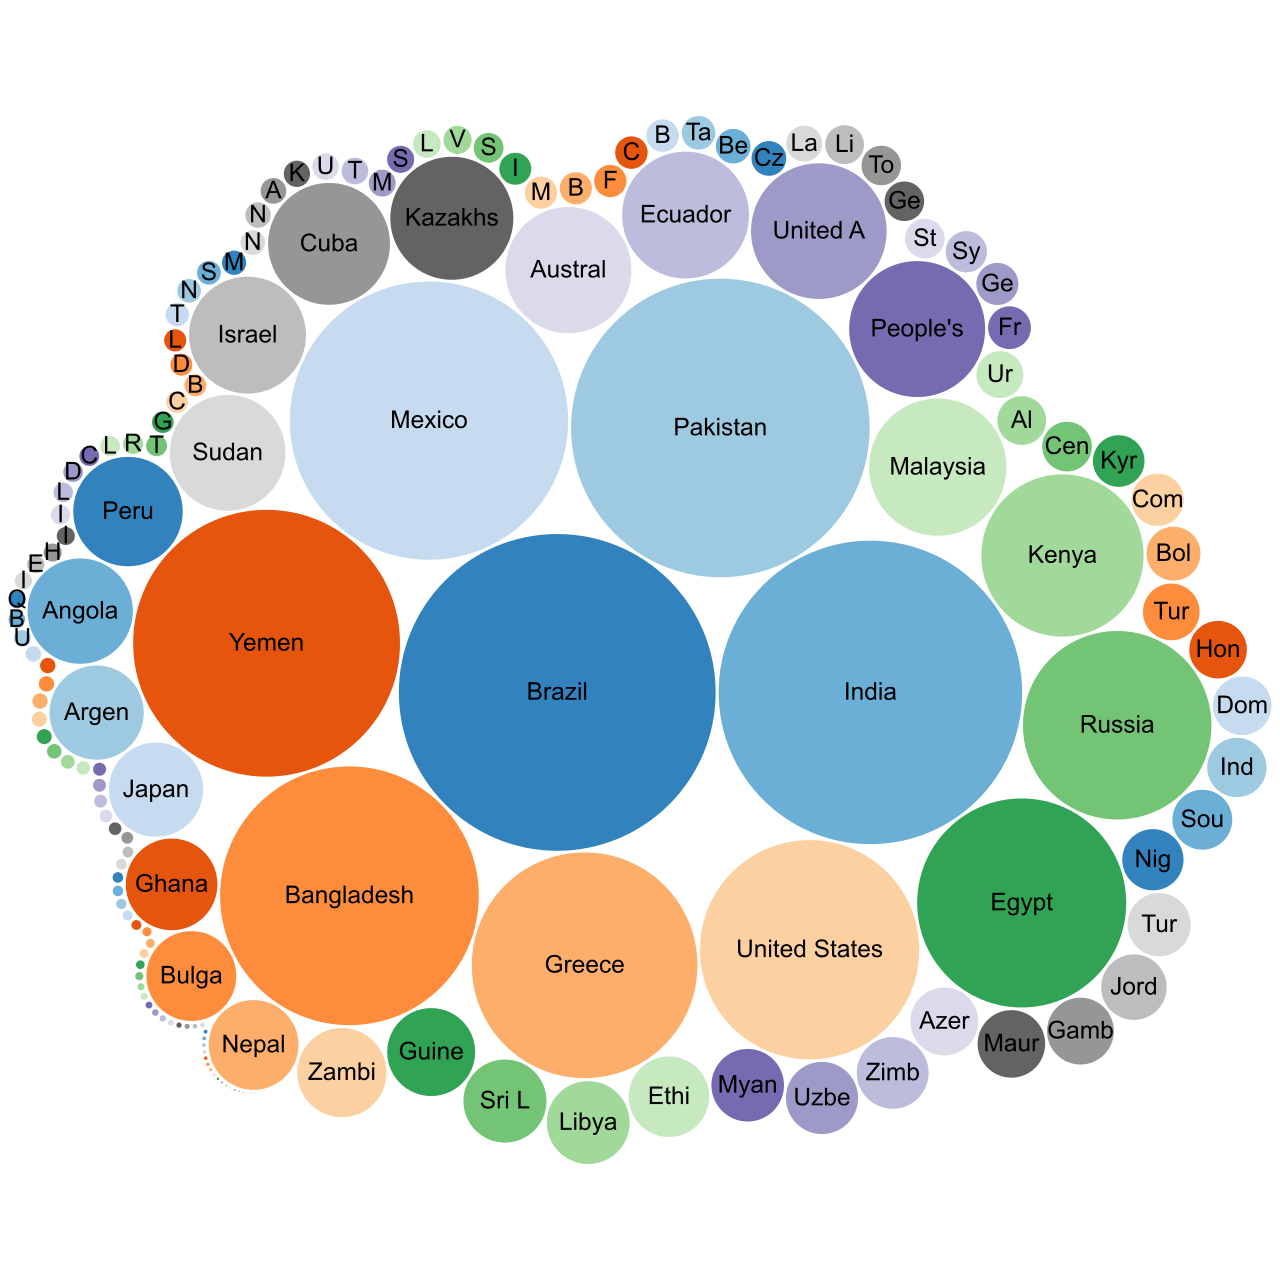
\includegraphics[width=0.9\linewidth]{./chapter/human_settlement/AnnaBubbleHumanSettlement.jpg}
	\label{fig:human-settlement-1}
    \caption[Bubble chart for the total population in ``human settlement'', 2017.] {Bubble chart for the total population living in ``human settlement'' for 2017. The size of the bubble corresponds to the number of people living in ``human settlement'' of one country. SPARQL query: \href{https://w.wiki/4f37}{https://w.wiki/4f37}}
\end{figure}

\begin{figure}
\centering
	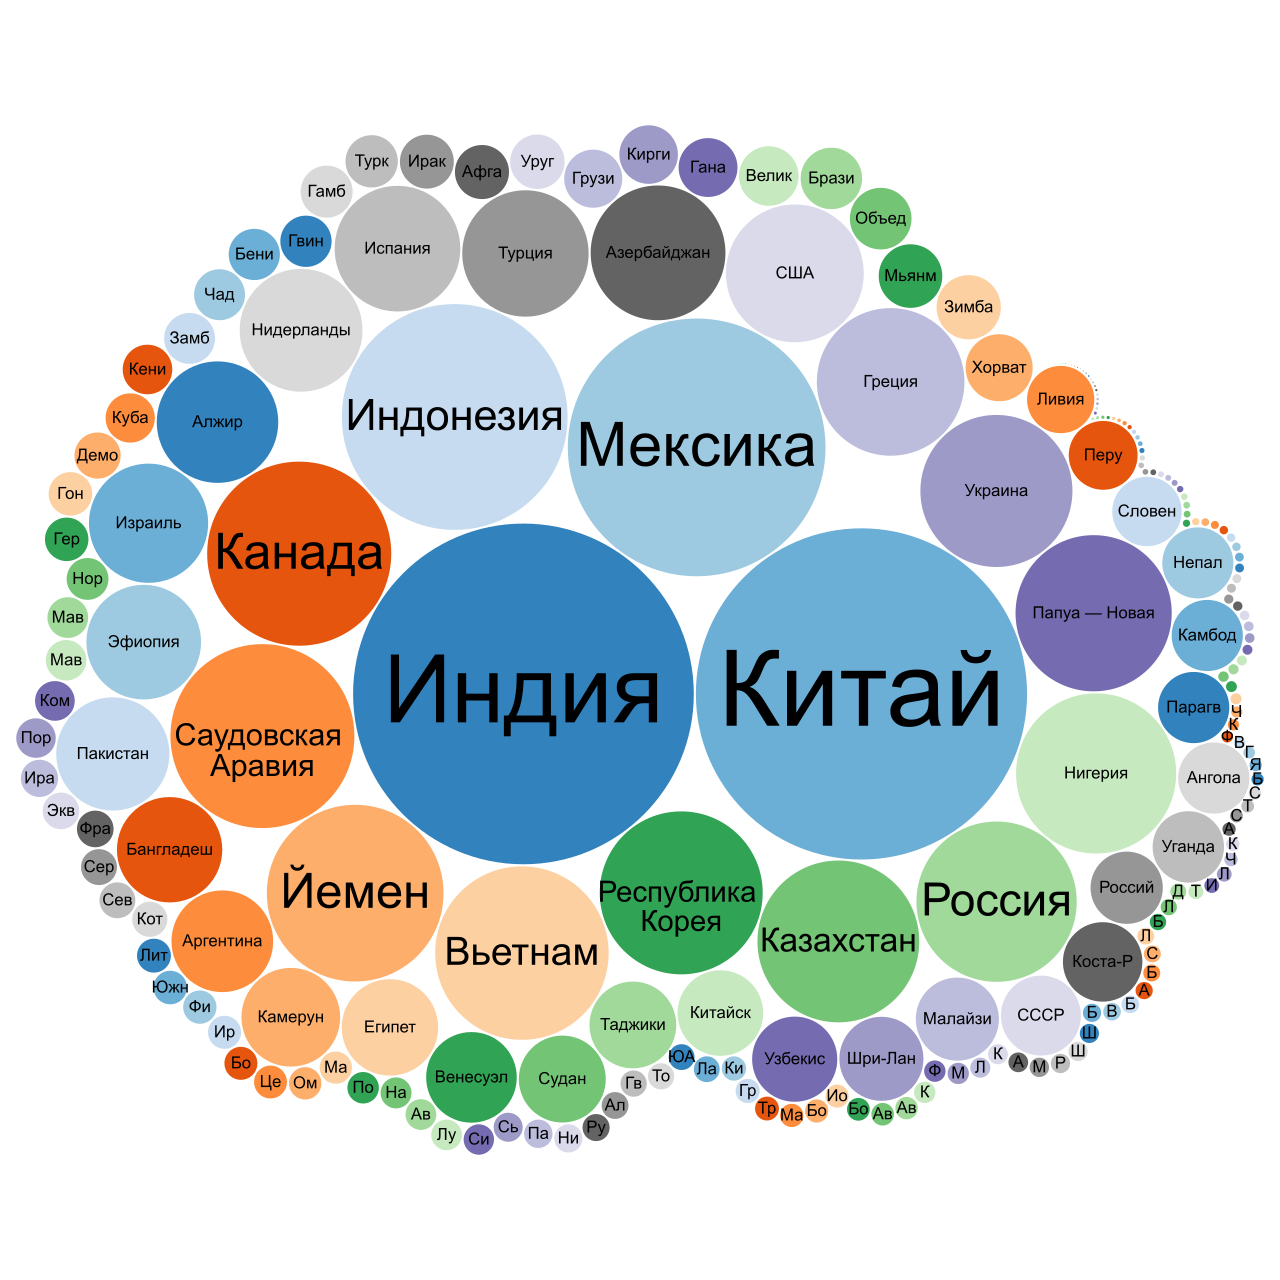
\includegraphics[width=0.9\linewidth]{./chapter/human_settlement/LeonidBubbleHumanSettlement.jpg}
	\label{fig:human-settlement-2}
	\caption[Bubble chart for the total population in ``human settlement'', 2021.] {Bubble chart for the total population living in ``human settlement'' for 2021. The size of the bubble corresponds to the number of people living in ``human settlement'' of one country. SPARQL query: \href{https://w.wiki/4f37}{https://w.wiki/4f37}}
\end{figure}

In 2017, most of the population lived in ``human settlement'':
\wdqName {Brazil} {155} (\num {12} millions),
\wdqName {Pakistan} {843} (\num {10} millions),
\wdqName {Mexico} {96} (\num {8} millions),
\wdqName {Yemen} {805} (\num {8} millions),
\wdqName {India} {668} (\num {7} millions) and
\wdqName {Bangladesh} {902} (\num{7} millions).

In Figure~\ref{fig:human-settlement-2}, you can see the list of countries for 2021:
\wdqName {India} {668} (\num {30} millions),
\wdqName {China} {148} (\num {28} millions),
\wdqName {Mexico} {96} (\num {17} millions),
\wdqName {Indonesia} {252} (\num {13} millions),
\wdqName {Canada} {16} (\num {9} millions) and
\wdqName {Saudi Arabia} {851} (\num {9} millions).

So, the results of the query~\ref{lst:human-settlement3} in 2017 and 2021 differ significantly.
Based on these results, it turns out that in four years
in the settlements of India has increased by 23 million people.

%%%%%
\subsection{Completeness of Wikidata}

Human settlement~--- is the common name for places with permanent residents\sidecite{Humansettlements_Dictionary}.
According to the editors of Wikidata, the concept of a locality includes cities, villages, hamlets
and others \marginnote [12pt] {The complete list can be seen in the section ``List of classes accompanying ``human settlement'' in the property ``instance of'''' on page~\pageref {human-settlement:tag1}.}.
Accurate information on the number of human settlements in the world was not found.
Therefore, we will check the completeness of the human settlements that are in Wikidata.
and which were used to solve the problem.
In the tasks above, we used the \wdProperty{1082}{population size} property and
\wdProperty{17}{state} (binding to the country).
Based on this, we divide the completeness check into subtasks:
\begin {enumerate}
  \item Check if the property ``population size'' is full.
  \item Check of attachment to the state.
\end {enumerate}

%%%%%
\subsection{Checking the occupancy of the property ``population''}

For such a check, write \href{https://w.wiki/4f3C}{SPARQL query}\sidenote {
%
In 2017, the request returned \num{372997} settlements
with the property ``population size'' empty.
The same request in 2021 yielded \num{507078} such settlements.
SPARQL query link: \href{https://w.wiki/4f3C}{https://w.wiki/4f3C}%
},
which will display settlements
with an empty property \href{http://www.wikidata.org/entity/P1082}{population size}.
Making calculations, we find that only 9.3\% of the world's settlements
the property ``population size'' for 2017 is indicated.
In 2021, we get 11.2\% of the world's settlements with a filled property ``population size''.
So, simultaneously with the increase in the number of settlements in Wikidata
he share of points with the filled property ``population size'' is growing.

%%%%%
\subsection{Verification of state supplies}

%%%%%%%%%%%%%%%%% Exercise 2 %%%%%%%%%%%%%%%%%%
\begin{marginfigure} [0.0 cm]
{
\includegraphics [width = 0.8\linewidth] {./chapter/human_settlement/Coat_of_Arms_of_Asbest_(Sverdlovsk_oblast).png}}
    \caption {Is this the emblem of a ``human settlement'' in Russia or other countries? \newline%
See~\protect\ref{answer:flag_human_settlements} on page~\protect\pageref{answer:flag_human_settlements}.}
    \label {fig:flag_question_human_settlements2}%
\end{marginfigure}

Now let's see the settlements,
in any country
using \href{https://w.wiki/4f3D}{SPARQL query} \footnote {%
%
In 2017, there were \num{8427} objects that did not include a record in any country.
In 2021, there are already more such objects~--- \num{27824}.

SPARQL query: \href{https://w.wiki/4f3D}{https://w.wiki/4f3D}%
}.

The query results show that the numeric value is not tied to a country that has been growing over the years.
Therefore, associated with settlements and countries,
not completely in terms of coverage, even relative to those already in Wikidata.

%%%%%
\section {Percentage of the country's population living in ``human settlement''}

Let's build an ordered list of countries in terms of the proportion of the population (in percent) living in \href{http://www.wikidata.org/entity/Q486972} {human settlements}, relative to the number of all inhabitants of the country (listing ~\ref{lst:human-settlement6}).

\index{SPARQL!SUM!The ratio of the number of people living in settlements to the number of all people in the country}
\begin{lstlisting}[ language=SPARQL, 
                    caption={The ratio of the number of people living in settlements to the number of all people in the country. The result contained \num{158} countries in 2017 and \num{206} countries in 2021. SPARQL query: \href{https://w.wiki/4f3H}{https://w.wiki/4f3H}},
                    label=lst:human-settlement6,
                    texcl 
                    ]
# An ordered list of the ratio of the number of people living in 
# "human\_settlement" to the number of inhabitants in the country.
SELECT ?country ?countryLabel ?proportionPopulation WHERE {
 SELECT ?country ?countryLabel (SUM(?population / ?pop) 
        as ?proportionPopulation) WHERE {
  ?hum wdt:P31 wd:Q486972;    # instances of human settlement  
       wdt:P17 ?country;         # has ?country 
       wdt:P1082 ?population.    # has ?population
  ?country wdt:P1082 ?pop.    # population in the country
  SERVICE wikibase:label{bd:serviceParam wikibase:language "en"}
 }
 GROUP BY ?country ?countryLabel
}
ORDER BY ?proportionPopulation
\end{lstlisting}%

The bar chart in Fig.~\ref{fig:human-settlement-3} allows you to see for each individual country the ratio of the number of people living in \href{http://www.wikidata.org/entity/Q486972}{human settlements}, to the number of inhabitants in the country for 2017.

\begin{figure*}
    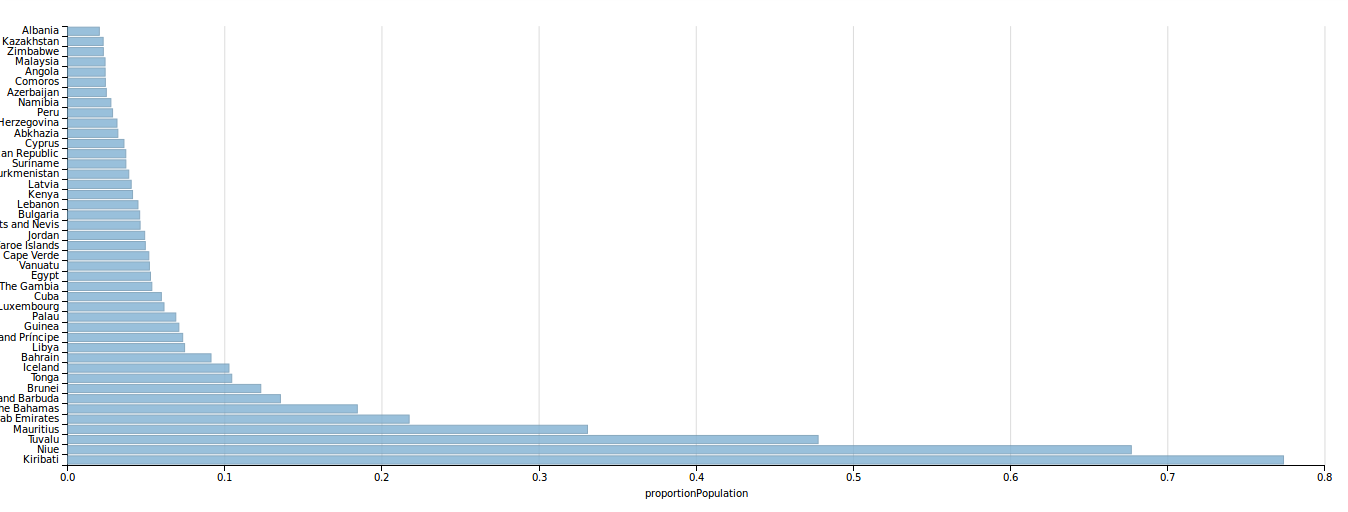
\includegraphics[width=\linewidth]{./chapter/human_settlement/AnnaShareHumanSettlement.png}
	\label{fig:human-settlement-3}
	\caption[Chart of the country's population share, 2017.]{Diagram of the share of the country's population living in ``human settlements'' for 2017. SPARQL query: \href{https://w.wiki/4f3H}{https://w.wiki/4f3H}}%
\end{figure*} 

\begin{figure*}
    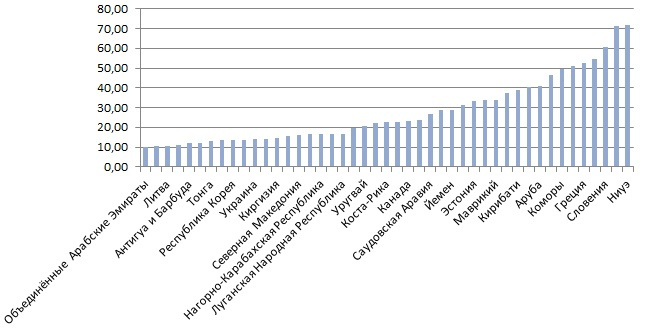
\includegraphics[width=\linewidth]{./chapter/human_settlement/LeonidShareHumanSettlement.jpg}
	\label{fig:human-settlement-4}
	\caption[Chart of the country's population share, 2021.]{Diagram of the share of the country's population living in ``human settlements'' for 2021. Countries with a population of more than 5 million people were selected. SPARQL query: \href{https://w.wiki/4f3K}{https://w.wiki/4f3K}}%
\end{figure*} 

%%%%%%%%%%%%%%%%% Exercise 2 %%%%%%%%%%%%%%%%%%
\begin{marginfigure} [0.0 cm]
{
\includegraphics [width = 0.9\linewidth] {./chapter/human_settlement/Aznakeevskii_rayon_gerb.png}}
    \caption {Is the coat of arms of a domestic or foreign human settlement shown in the picture? \newline%
See~\protect\ref{answer:flag_human_settlements} on page~\protect\pageref{answer:flag_human_settlements}.}
    \label {fig:flag_question_human_settlements1}%
\end{marginfigure}

According to Fig.~\ref{fig:human-settlement-3} it can be seen
that the following countries accounted for the highest percentage in 2017: 
Kiribati (78\%), Niue (70\%), Greece (53\%), Tuvalu (48\%), Comoros (43\%), Mauritius (42\%). 
In 2021, the picture has changed: Nigeria (93\%), Papua~--- New Guinea (71\%),
Israel (50\%), Greece (47\%), Azerbaijan (47\%), Kazakhstan (37\%). 
Note that these are mostly small island states. 
Probably, most of the inhabitants of these countries are concentrated in populated areas.

As of 2017 , the share of residents in the G8 countries 
in \href{http://www.wikidata.org/entity/Q486972}{human settlements} made up: 
\href{http://www.wikidata.org/entity/Q159}{Russia} (\num{2.98}\%), 
\href{http://www.wikidata.org/entity/Q30 }{USA} (\num{1.76}\%), 
\href{http://www.wikidata.org/entity/Q17}{Japan} (\num{0.80}\%), 
\href{http://www.wikidata.org/entity/Q16}{Canada} (\num{0.26}\%), 
\href{http://www.wikidata.org/entity/Q142 }{France} (\num{0.20}\%), 
\href{http://www.wikidata.org/entity/Q183 }{Germany} (\num{0.24}\%), 
\href{http://www.wikidata.org/entity/Q145 }{UK} (\num{0.18}\%), 
\href{http://www.wikidata.org/entity/Q38}{Italy} (\num{0.07}\%). 
In 2021, the values of the population share decreased (Fig.~\ref{fig:human-settlement-4}):
\href{http://www.wikidata.org/entity/Q159 }{Russia} (0.045\%), 
\href{http://www.wikidata.org/entity/Q30 }{USA} (\num{0.014}\%), 
\href{http://www.wikidata.org/entity/Q17}{Japan} (\num{0.008}\%), 
\href{http://www.wikidata.org/entity/Q16}{Canada} (\num{0.23}\%), 
\href{http://www.wikidata.org/entity/Q142 }{France} (\num{0.005}\%), 
\href{http://www.wikidata.org/entity/Q183 }{Germany} (\num{0.005}\%), 
\href{http://www.wikidata.org/entity/Q145 }{UK} (\num{0.014}\%), 
\href{http://www.wikidata.org/entity/Q38}{Italy} (\num{0.0005}\%). 
Note that these are industrialized countries.

The constructed diagram confirms the following hypothesis:
a high percentage of the country's population living in ``human settlements'', 
indicates a more agrarian country. 
From diagrams~\ref{fig:human-settlement-3} and ~\ref{fig:human-settlement-4} it can be seen
that the highest percentage of the country's population living in settlements
falls on island, southern, hot countries,
in which, apparently, industry is less developed 
(small territory, small population, distance from the continents). 
And the industrial countries (the Big Eight) have a very low percentage of the country's population
living in populated areas.

%%%%%
\section{List of classes accompanying ``human settlements'' in ~property ``instance of''}
\label{human-settlement:tag1}

We will call ``class'' such Wikidata objects
that are associated with any Wikidata object through the \wdProperty{31}{instance of}.
The purpose of this section is~--- to find $X$ objects
for which the object \wdqName{human settlement}{486972} is a class,
and to get other classes of the object $X$, except ``human settlement''.
These ``other'' classes will be called accompanying ``human settlement''.
With a request~\ref{lst:human-settlement7}
we will find the objects accompanying ``human settlement''.

\begin{lstlisting}[ language=SPARQL,
    caption={List of classes accompanying the ``human settlement''  (instance of). The result contained \num{610} in 2017 and \num{1245} in 2021. SPARQL query:\href{https://w.wiki/4f3Q}{https://w.wiki/4f3Q}}, 
    label=lst:human-settlement7,
    texcl 
                  ]
# List of classes accompanying the human\_settlement (instance of)
SELECT ?inst (COUNT(?hum) as ?sumHum) 
WHERE{          
  ?hum wdt:P31 wd:Q486972; # instance of human settlement
       wdt:P31 ?inst.      # other objects in instance
  SERVICE wikibase:label{bd:serviceParam wikibase:language "en"}
}  
GROUP BY ?inst
\end{lstlisting}%

%%%%%%%%%%%%%%%%% Exercise 2 %%%%%%%%%%%%%%%%%%
\begin{marginfigure} [0.0 cm]
{
\includegraphics[width=0.9\linewidth]{./chapter/human_settlement/Coat_of_Arms_of_Azov.png}}
    \caption {The coat of arms of the ``human settlement''  of which country is depicted? \newline%
See~\protect\ref{answer:flag_human_settlements} on page~\protect\pageref{answer:flag_human_settlements}.}
    \label {fig:flag_question_human_settlements5}%
\end{marginfigure}

To speed up the execution of the request~\ref{lst:human-settlement7} let's do two steps.

First, we will turn off the settlement from consideration, 
having only ``human settlement'' in the ~list of instances,
since there are no other related classes. 
To do this, add the line ~\num{9} to the script~\ref{lst:human-settlement8} with a filter
requiring that the object \lstinline|?hum| 
except \wdProperty{31}{instance} ``human settlement'' there was another class.

Secondly, in the line \num{8} requests~\ref{lst:human-settlement8}
removing such objects of the variable \lstinline|?insert|, 
which have the property \wdqName{state}{17}. 
This will allow you to cut off hundreds of types of settlements specific to individual countries, 
for example, ``administrative-territorial unit of Russia''.

These transformations made it possible to execute the query~\ref{lst:human-settlement8}
for all countries of the world in an acceptable time of 13 ms.

\begin{lstlisting}[ language=SPARQL, 
    caption={List of classes associated with ``human settlement" in the ``instance of" property without specialized classes of different countries. The result contained \num{355} in 2017 and \num{707} in 2021. SPARQL query:\href{https://w.wiki/4f3U}{https://w.wiki/4f3U}}, 
    label=lst:human-settlement8,
    texcl 
                  ]
# List of objects with the class of human settlement, without 
# country and single human settlement
SELECT ?inst ?instLabel (COUNT(?hum) as ?sumHum) 
WHERE{ 
  ?hum wdt:P31 wd:Q486972;  # instance of human settlement
       wdt:P31 ?inst.       # other objects in instance
  
  MINUS {?inst wdt:P17 []}. # without country
  FILTER(?inst != wd:Q486972 ). # without human settlement
  SERVICE wikibase:label{bd:serviceParam wikibase:language "en"}
}  
GROUP BY ?inst ?instLabel
ORDER BY DESC (?sumHum)
\end{lstlisting}%

The table~\ref{tab:human-settlement2} presents
comparative results for 2017 and 2021,
the number of classes associated with ``human settlement" in the ``instance of" property.

\begin{table}[h]
\centering
\begin{tabular}{|l|l|l|l|l|}
\hline
\textnumero & Class name     & 2017 & 2021 & $\Delta$ \\ \hline
1 & \wdqName{Village}{532} & \num{2844} & \num{4853} & +\num{2009}	\\
2 & \wdqName{Municipalities}{15284} & \num{1181} & \num{3376} & +\num{2195} \\
3 & \wdqName{Villages}{5084} & \num{662} & \num{1761} &+\num{1099}	\\ 
4 & \wdqName{Archaeological sites}{839954} & \num{425} & \num{887} & +\num{462} \\
5 & \wdqName{Local settlements}{3257686} & \num{425} & \num{158} & -\num{257}	\\ 
6 & \wdqName{Destroyed cities}{14616455} & \num{423} & \num{388} & -\num{40}	\\
7 & \wdqName{Cities}{515} & \num{322} & \num{545} & +\num{223} \\
8 & \wdqName{Small Towns}{3957} & \num{277} & \num{446} & +\num{169} \\
9 & \wdqName{Abandoned Villages}{350895} & \num{254} & \num{474} & +\num{220}	\\ 
10 & \wdqName{Hinterland}{2983893} & \num{207} & \num{503} & +\num{296} \\\hline
\end{tabular}
\caption{The number of classes accompanying ``human settlement" in~2017 and 2021, their difference ($\Delta$).}
\label{tab:human-settlement2}
\end{table}

The query~\ref{lst:human-settlement8} showed that in 2021, 
prehistoric settlements of three types were in the first places among the classes accompanying ``human settlement"
: settlements
\wdqName{Laten period}{106505016}, 
\wdqName{Bronze Age}{106491277} 
and settlements \wdqName{prehistoric time, where there is writing}{106505070}. 

Let's try to formulate the request in such a way as to cut off all the many prehistoric settlements.  
What do these three objects on Wikidata have in common? 
They are instances of objects that, in turn,
are instances of objects \wdqName{archaeological culture}{465299}, 
\wdqName{historical period}{11514315}, 
\wdqName{archaeological age}{15401699}, 
\wdqName{world history}{200325} 
and \wdqName{geological period}{392928}. 
Let's apply such a filter in the request~\ref{lst:human-settlement9} in lines 10--12
to cut off exactly these types of objects.

\index{SPARQL!COUNT!List of classes associated with ``human settlements'' in ~property ``instance of'', without historical objects}
\index{SPARQL!FILTER!List of classes associated with ``human settlements'' in ~property ``instance of'', without historical objects}
\index{SPARQL!MINUS!List of classes associated with ``human settlements'' in ~property ``instance of'', without historical objects}
\begin{lstlisting}[ language=SPARQL,
    caption={List of classes associated with ``human settlements'' in ~property ``instance of'', without historical objects. The result contained \num{89} in 2021. SPARQL query:\href{https://w.wiki/4f3W}{https://w.wiki/4f3W}}, 
                    label=lst:human-settlement9,
                    texcl 
                    ]
# List of classes accompanying the human\_settlement in the property
# 'instance of' without historical objects 
SELECT ?inst ?instLabel (COUNT(?hum) as ?sumHum) WHERE{
  ?hum wdt:P31 wd:Q486972;    # instance of human settlement
       wdt:P31 ?inst. # other objects in instance of human settlement
  ?inst wdt:P31 ?test. # instance of ?inst
  ?test wdt:P31 ?typ. # instance of ?test
  MINUS {?inst wdt:P17 []}.   # without country
  # without human settlement and prehistoric settlements
  FILTER(?inst != wd:Q486972 && ?typ != wd:Q465299 
         && ?typ != wd:Q11514315 && ?typ != wd:Q15401699 
         && ?typ != wd:Q200325 && ?typ != wd:Q392928 ). 
  SERVICE wikibase:label{bd:serviceParam wikibase:language "en"}
}
GROUP BY ?inst ?instLabel
ORDER BY DESC (?sumHum)
\end{lstlisting}%

%%%%%%%%%%%%%%%%% Exercise 2 %%%%%%%%%%%%%%%%%%
\begin{marginfigure} [0.0 cm]
{
\includegraphics [width = 0.8\linewidth] {./chapter/human_settlement/Loučovice_CoA.jpg}}
    \caption {The coat of arms of the ``human settlement'' of which country is depicted? \newline%
See~\protect\ref{answer:flag_human_settlements} on page~\protect\pageref{answer:flag_human_settlements}.}
    \label {fig:flag_question_human_settlements3}%
\end{marginfigure}

As a result, 706 query classes~\ref{lst:human-settlement7} 
we have shortened in~request~\ref{lst:human-settlement8} 
up to 89 different classes associated with ``human settlements'' in ~property ``instance of''.

%%%%%
\section{Domestic scientists in the countryside and in the city}

Let's calculate and compare the number of Russian scientists born in rural and town types of settlements. 
Let's solve this problem in five steps:

%%%%%%%%%%%%%%%%% Exercise 2 %%%%%%%%%%%%%%%%%%
\begin{marginfigure} [0.0 cm]
{
\includegraphics[width=0.9\linewidth]{./chapter/human_settlement/POL_Otynia_COA.png}}
    \caption {The coat of arms of the ``human settlement'' of which country is depicted? \newline%
See~\protect\ref{answer:flag_human_settlements} on page~\protect\pageref{answer:flag_human_settlements}.}
    \label {fig:flag_question_human_settlements4}%
\end{marginfigure}

\begin{enumerate}
\item We will identify a list of rural and a list of town settlement types in Russia.
\item We will define the main scientific directions presented in ~Wikidata.
\item We will identify a way to identify domestic scientists.
\item We will make such a diagram on which different scientific directions (mathematicians, physicists, chemists, and so on) will be indicated in different colors for scientists born in rural settlements.
\item Let's make a second diagram~--- by town settlements and compare the results.
\end{enumerate}

%%%%%
\subsection{List of rural and list of town settlement types in~Russia}

Output a list of settlement classes and their number for objects, 
having the property \wdProperty{1082}{population size}
and belonging to \wdqName{Russia}{159} (listing~\ref{lst:human-settlement4}).

\index{SPARQL!COUNT!List of settlement classes and their number for objects having the property ``population size'' in Russia}
\begin{lstlisting}[ language=SPARQL, 
    caption={List of settlement classes and their number for objects having the property ``population size'' in Russia. The result contained \num{216} in 2021. SPARQL query:\href{https://w.wiki/4f3Y}{https://w.wiki/4f3Y}}, 
                    label=lst:human-settlement4,
                    texcl 
                    ]
# List of settlement classes and their number for objects with 
# the property "population" in Russia
SELECT ?class ?classLabel (COUNT(?class) AS ?count) WHERE {
  {
  SELECT ?class ?classLabel ?humLabel WHERE {
   ?hum wdt:P17 wd:Q159;  # settlement in the Russia
        wdt:P1082 ?population; # has ?population
        wdt:P31 ?class. # has ?class
    SERVICE wikibase:label{bd:serviceParam wikibase:language "en"}
   }
  }
}
GROUP BY ?class ?classLabel
ORDER BY DESC (?count)
\end{lstlisting}%

The main classes obtained by the request~\ref{lst:human-settlements4}, are presented in the table~\ref{tab:human-settlement1}.

\begin{table}[h]
\centering
\begin{tabular}{|l|l|l|l|}
\hline
number & class name                     						& number of mentions	& population size		\\ \hline
1 & \wdqName{rural settlement in Russia}{634099} & \num{18104} & \num{34043885} 		\\
2 & \wdqName{hamlet}{5084} & \num{14795} & \num{1727221}       	\\
3 & \wdqName{village}{532} & \num{9875} & \num{10584016} 		\\ 
4 & \wdqName{posyolok}{2514025} & \num{4418} & \num{3326567} 		\\ 
7 & \wdqName{farm}{2023000} & \num{1733} & \num{509825} 		\\ 
9 & \wdqName{city}{7930989} & \num{1171} & \num{104453583} 	\\ 
10 & \wdqName{human settlement}{486972} & \num{1168} & \num{6643211} 		\\ 
11 & \wdqName{Russian urban-type settlement}{15078955} & \num{665} & \num{3745723} 		\\ 
21 & \wdqName{city with population over 100,000}{1549591} & \num{108} & \num{58159327} 		\\ 
54 & \wdqName{million city}{1637706} & \num{14} & \num{32136227} \\\hline
\end{tabular}
\caption{Table of classes and their number of mentions among objects having the property ``population size'' in Russia}
\label{tab:human-settlement1}
\end{table}

The studies conducted above show that the ``human settlements'' class is used in conjunction with different classes of settlements. Therefore, we will not add it to either rural or town settlements.

Next, the classes from the table~\ref{tab:human-settlement1} are numbered: 1, 2, 3, 4 and 7. In the future, the combination of these classes will be referred to as rural settlements. Let's calculate the number of the population of such settlements in Russia\footnote{Received 50 million people. Link to SPARQL query: \href{https://w.wiki/4f3b}{https://w.wiki/4f3b}}.

And the classes from the table~\ref{tab:human-settlement1} are numbered: 9, 11, 21 and 54. In the future, the combination of these classes will be referred to as town settlements. Let's calculate the number of the population of such settlements in Russia\footnote{Received 198 million people. Link to SPARQL query: \href{https://w.wiki/4f3f}{https://w.wiki/4f3f}}.

%%%%%
\subsection{The main scientific directions presented in Wikidata}

Output a list of professions and their number for people with the property \wdProperty{27}{citizenship} \wdqName{Russia}{159} (listing~\protect\ref{lst:human-settlement13}).

\index{SPARQL!COUNT!List of occupation or job citizens of Russia }
\lstset{numbers=left, firstnumber=1, frame=single}
\begin{lstlisting}[ language=SPARQL,
    caption={List of occupation or job citizens of Russia. The result contained \num{89} in 2021. SPARQL query:\href{https://w.wiki/4f3h}{https://w.wiki/4f3h}},  
                    label=lst:human-settlement13,
                    texcl 
                    ]
# List of occupation or job citizens of Russia 
SELECT DISTINCT ?job ?jobLabel (COUNT(?hum) AS ?count) WHERE {
  ?hum wdt:P27 wd:Q159; # citizen of Russia 
       wdt:P106 ?job. # has occupation or job
  SERVICE wikibase:label{bd:serviceParam wikibase:language "ru,en"}
}
GROUP BY ?job ?jobLabel
ORDER BY ?count
\end{lstlisting}%

Below is a table~\ref{tab:human-settlement3} with selected scientific directions from (listing~\protect\ref{lst:human-settlement13}).

\begin{table}[h]
\centering
\begin{tabular}{|l|l|l|}
\hline
number & class name      					& number of mentions	\\ \hline
1 & \wdqName{physicist}{169470} & \num{991}                		\\
2 & \wdqName{historian}{201788} & \num{913}                		\\
3 & \wdqName{economist}{188094} & \num{880}               		\\ 
4 & \wdqName{mathematician}{170790} & \num{857}               		\\ 
5 & \wdqName{engineer}{81096} & \num{558}               		\\ 
6 & \wdqName{researcher}{1650915} & \num{502}               		\\ 
7 & \wdqName{chemist}{593644} & \num{439}               		\\ 
8 & \wdqName{doctor}{39631} & \num{342}               		\\ 
9 & \wdqName{lawyer}{185351} & \num{330}               		\\ 
10 & \wdqName{biologist}{864503} & \num{222} \\\hline
\end{tabular}
\caption{Table of scientific directions and their number of mentions among people with Russian citizenship}
\label{tab:human-settlement3}
\end{table}

%%%%%
\subsection{To identify a way to identify domestic scientists}

There are two ways to get a list of scientists. 
The first by the presence of the property \wdProperty{512}{scientific degree}. 
Output a list of people with this property (listing~\protect\ref{lst:human-settlement14}).

\index{SPARQL!COUNT!Count of peoples in Russian with academic degree}
\begin{lstlisting}[ language=SPARQL,
    caption={Count of peoples in Russian with academic degree. The result contained \num{24297} in 2021. SPARQL query:\href{https://w.wiki/4f3i}{https://w.wiki/4f3i}},  
                    label=lst:human-settlement14,
                    texcl 
                    ]
# Count of peoples in Russian with academic degree
SELECT (COUNT(DISTINCT ?hum) AS ?human_count) WHERE {
  # Russian Empire, Soviet Union and Russia
  VALUES ?ruCountries {wd:Q34266 wd:Q15180 wd:Q159}
  ?hum wdt:P512 ?academic_degree;  # has academic degree 
       wdt:P27 ?ruCountries. # lives (lived) in Russian countries
  SERVICE wikibase:label{bd:serviceParam wikibase:language "en"}
}
\end{lstlisting}%

The second property \wdProperty{463}{member of the organization} of several academies: \wdqName{academy of sciences}{414147}, \wdqName{learned society}{955824}, \wdqName{scientific society}{74801}, \wdqName{academy}{162633}, \wdqName{research institute}{31855}, \wdqName{educational institution}{2385804}. Output a list of people with this property (listing~\protect\ref{lst:human-settlement15}).

\index{SPARQL!COUNT!Count of peoples in Russian in academy}
\begin{lstlisting}[ language=SPARQL, 
    caption={Count of peoples in Russian in academy. The result contained \num{24297} in 2021. The result contained \num{4170} in 2021. SPARQL query:\href{https://w.wiki/4f3n}{https://w.wiki/4f3n}},
                    label=lst:human-settlement15,
                    texcl 
                    ]
# Count of peoples in Russian in academy
SELECT (COUNT(DISTINCT ?hum) AS ?human_count) WHERE {
  VALUES ?ruCountries {wd:Q34266 wd:Q15180 wd:Q159}
  VALUES ?class_academy {wd:Q414147 wd:Q955824 wd:Q74801 wd:Q162633 
                      wd:Q31855 wd:Q2385804 wd:Q83172}
  ?hum wdt:P463 ?academy;  # has academic degree 
       wdt:P27 ?ruCountries. # lives (lived) in countries
  # academy is an element of the class academy
  ?academy wdt:P31 ?class_academy. 
  SERVICE wikibase:label{bd:serviceParam wikibase:language "en"}
}
\end{lstlisting}%

The first method gives more people, which will allow you to see a more detailed picture in the diagrams below. We will use it to build diagrams below.

%%%%%
\subsection{Construction of a diagram on which different scientific directions will be indicated in different colors for scientists born in rural settlements}

Using the steps described above, we get the request~\protect\ref{lst:human-settlement16}.

\index{SPARQL!COUNT!Diagram of the number of scientists by occupation in rural settlements}
\index{SPARQL!FILTER!Diagram of the number of scientists by occupation in rural settlements}
\index{SPARQL!FLOOR!Diagram of the number of scientists by occupation in rural settlements}
\index{SPARQL!YEAR!Diagram of the number of scientists by occupation in rural settlements}
\index{SPARQL!STR!Diagram of the number of scientists by occupation in rural settlements}
\index{SPARQL!BIND!Diagram of the number of scientists by occupation in rural settlements}
\index{SPARQL!GROUP BY!Diagram of the number of scientists by occupation in rural settlements}
\index{Chart!BarChart!Diagram of the number of scientists by occupation in rural settlements}

\begin{lstlisting}[ language=SPARQL, 
    caption={Diagram of the number of scientists by occupation in town settlements. SPARQL query: \href{https://goo.su/a3FT}{https://goo.su/a3F}},
                    label=lst:human-settlement16,
                    texcl 
                    ]
# defaultView:BarChart
# Diagram of the number of scientists by occupation in rural settlements

\end{lstlisting}%

The diagram~\ref{fig:human-settlement-5} shows the number of scientists by occupation
born in rural settlements.

\begin{figure*}
    \setlength{\fboxsep}{0pt}%
    \setlength{\fboxrule}{1pt}%
    \fcolorbox{gray}{gray}{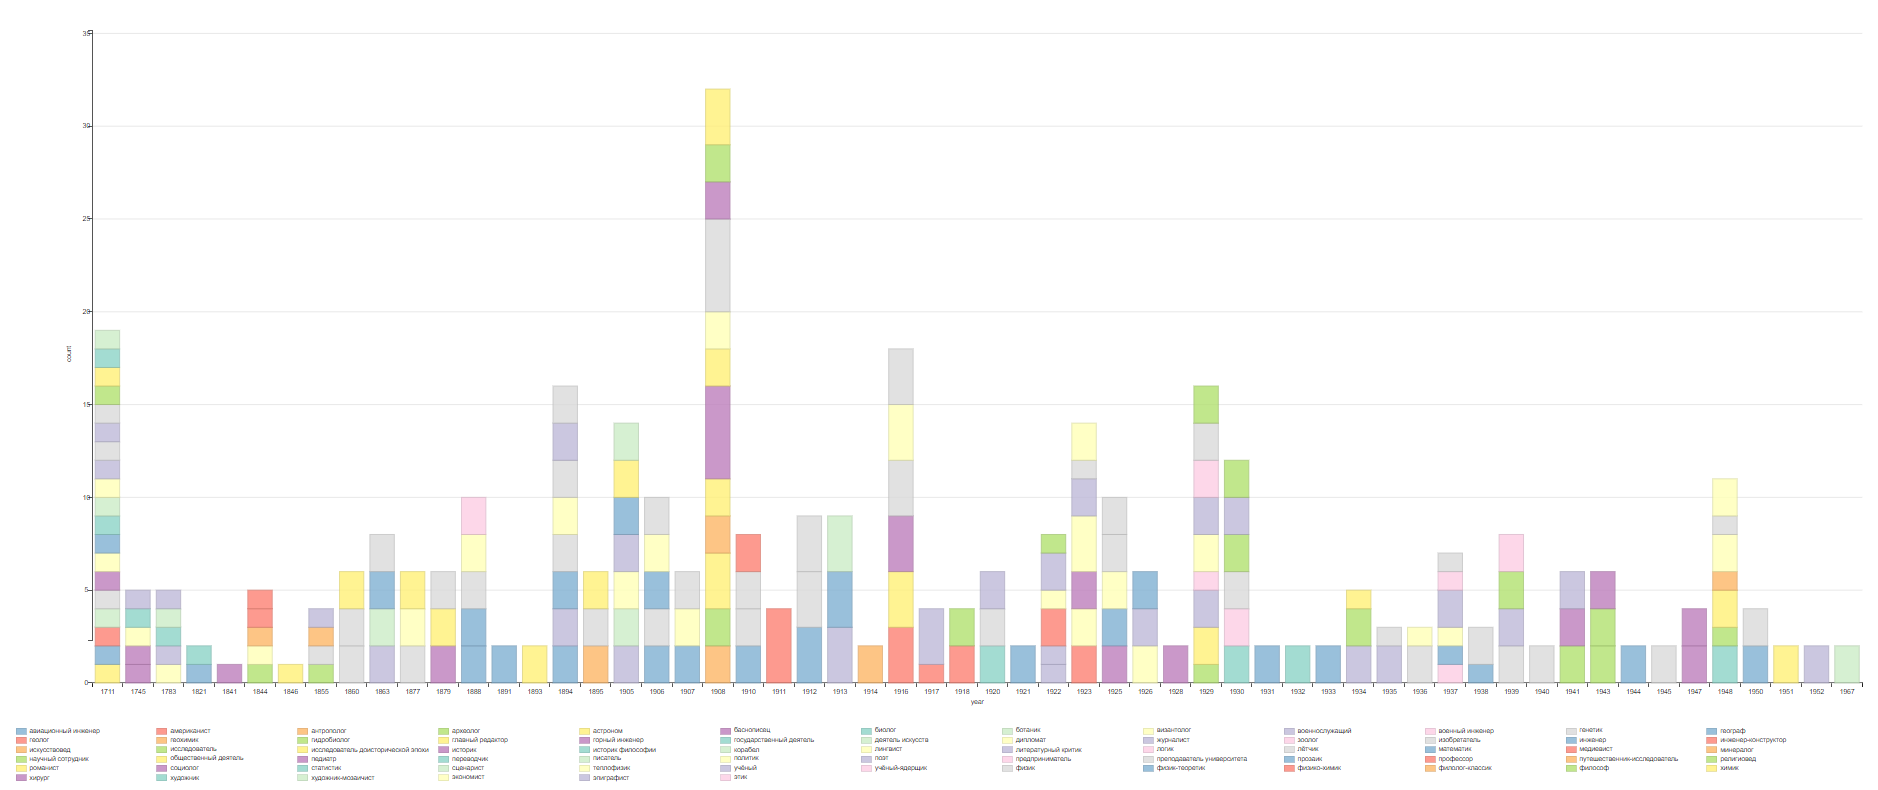
\includegraphics[width=1\linewidth]{./chapter/human_settlement/RussianScientistBornVillage.png}}
	\label{fig:human-settlement-5}
	\caption[Diagram of the number of scientists by occupation in rural settlements.]{Diagram of the number of scientists by occupation in rural settlements. SPARQL query: \href{https://goo.su/a3FT}{https://goo.su/a3F}}%
\end{figure*} 

%%%%%
\subsection{Plotting diagrams for scientists born in town settlements and comparing diagrams}

Using the steps described above, we get such a request~\ref{lst:human-settlement17}.

\index{SPARQL!COUNT!Diagram of the number of scientists by occupation in town settlements}
\index{SPARQL!FILTER!Diagram of the number of scientists by occupation in town settlements}
\index{SPARQL!FLOOR!Diagram of the number of scientists by occupation in town settlements}
\index{SPARQL!YEAR!Diagram of the number of scientists by occupation in town settlements}
\index{SPARQL!STR!Diagram of the number of scientists by occupation in town settlements}
\index{SPARQL!BIND!Diagram of the number of scientists by occupation in town settlements}
\index{SPARQL!GROUP BY!Diagram of the number of scientists by occupation in town settlements}
\index{Chart!BarChart!Diagram of the number of scientists by occupation in town settlements}

\begin{lstlisting}[ language=SPARQL, 
    caption={Diagram of the number of scientists by occupation in town settlements. SPARQL query: \href{https://goo.su/a9U0}{https://goo.su/a9U0}},
                    label=lst:human-settlement17,
                    texcl 
                    ]
# defaultView:BarChart
# Diagram of the number of scientists by occupation in town settlements

\end{lstlisting}%

The diagram~\ref{fig:human-settlement-6} shows the number of scientists by occupation born in town woodlands.

\begin{figure*}
    \setlength{\fboxsep}{0pt}%
    \setlength{\fboxrule}{1pt}%
    \fcolorbox{gray}{gray}{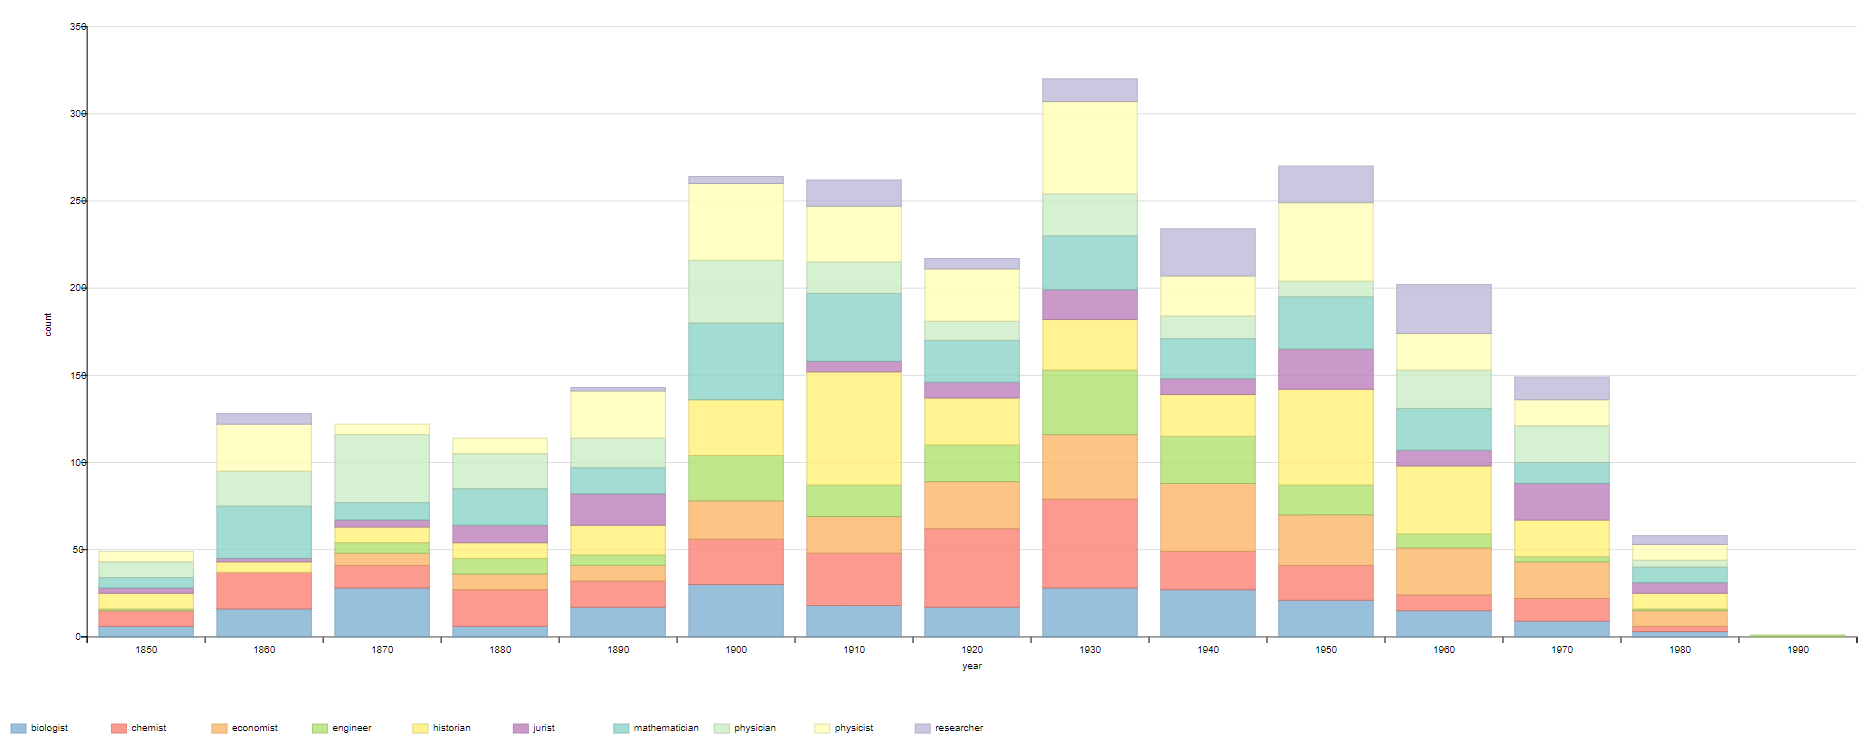
\includegraphics[width=1\linewidth]{./chapter/human_settlement/RussianScientistBornTown.png}}
	\label{fig:human-settlement-6}
	\caption[Diagram of the number of scientists by occupation in town settlements.]{Diagram of the number of scientists by occupation in town settlements. SPARQL query: \href{https://goo.su/a9U0}{https://goo.su/a9U0}}%
\end{figure*} 

Comparing the diagrams, it can be seen that there are about 3 times more scientists in town settlements than in rural settlements. Above, we counted the number of people from these groups, the difference in population reaches almost 4 times. Therefore, we can say that it does not matter where you were born.
